% Options for packages loaded elsewhere
% Options for packages loaded elsewhere
\PassOptionsToPackage{unicode}{hyperref}
\PassOptionsToPackage{hyphens}{url}
\PassOptionsToPackage{dvipsnames,svgnames,x11names}{xcolor}
%
\documentclass[
  american,
  letterpaper,
  DIV=11,
  numbers=noendperiod]{scrartcl}
\usepackage{xcolor}
\usepackage{amsmath,amssymb}
\setcounter{secnumdepth}{5}
\usepackage{iftex}
\ifPDFTeX
  \usepackage[T1]{fontenc}
  \usepackage[utf8]{inputenc}
  \usepackage{textcomp} % provide euro and other symbols
\else % if luatex or xetex
  \usepackage{unicode-math} % this also loads fontspec
  \defaultfontfeatures{Scale=MatchLowercase}
  \defaultfontfeatures[\rmfamily]{Ligatures=TeX,Scale=1}
\fi
\usepackage{lmodern}
\ifPDFTeX\else
  % xetex/luatex font selection
\fi
% Use upquote if available, for straight quotes in verbatim environments
\IfFileExists{upquote.sty}{\usepackage{upquote}}{}
\IfFileExists{microtype.sty}{% use microtype if available
  \usepackage[]{microtype}
  \UseMicrotypeSet[protrusion]{basicmath} % disable protrusion for tt fonts
}{}
\makeatletter
\@ifundefined{KOMAClassName}{% if non-KOMA class
  \IfFileExists{parskip.sty}{%
    \usepackage{parskip}
  }{% else
    \setlength{\parindent}{0pt}
    \setlength{\parskip}{6pt plus 2pt minus 1pt}}
}{% if KOMA class
  \KOMAoptions{parskip=half}}
\makeatother
% Make \paragraph and \subparagraph free-standing
\makeatletter
\ifx\paragraph\undefined\else
  \let\oldparagraph\paragraph
  \renewcommand{\paragraph}{
    \@ifstar
      \xxxParagraphStar
      \xxxParagraphNoStar
  }
  \newcommand{\xxxParagraphStar}[1]{\oldparagraph*{#1}\mbox{}}
  \newcommand{\xxxParagraphNoStar}[1]{\oldparagraph{#1}\mbox{}}
\fi
\ifx\subparagraph\undefined\else
  \let\oldsubparagraph\subparagraph
  \renewcommand{\subparagraph}{
    \@ifstar
      \xxxSubParagraphStar
      \xxxSubParagraphNoStar
  }
  \newcommand{\xxxSubParagraphStar}[1]{\oldsubparagraph*{#1}\mbox{}}
  \newcommand{\xxxSubParagraphNoStar}[1]{\oldsubparagraph{#1}\mbox{}}
\fi
\makeatother

\usepackage{color}
\usepackage{fancyvrb}
\newcommand{\VerbBar}{|}
\newcommand{\VERB}{\Verb[commandchars=\\\{\}]}
\DefineVerbatimEnvironment{Highlighting}{Verbatim}{commandchars=\\\{\}}
% Add ',fontsize=\small' for more characters per line
\newenvironment{Shaded}{}{}
\newcommand{\AlertTok}[1]{\textcolor[rgb]{1.00,0.00,0.00}{\textbf{#1}}}
\newcommand{\AnnotationTok}[1]{\textcolor[rgb]{0.38,0.63,0.69}{\textbf{\textit{#1}}}}
\newcommand{\AttributeTok}[1]{\textcolor[rgb]{0.49,0.56,0.16}{#1}}
\newcommand{\BaseNTok}[1]{\textcolor[rgb]{0.25,0.63,0.44}{#1}}
\newcommand{\BuiltInTok}[1]{\textcolor[rgb]{0.00,0.50,0.00}{#1}}
\newcommand{\CharTok}[1]{\textcolor[rgb]{0.25,0.44,0.63}{#1}}
\newcommand{\CommentTok}[1]{\textcolor[rgb]{0.38,0.63,0.69}{\textit{#1}}}
\newcommand{\CommentVarTok}[1]{\textcolor[rgb]{0.38,0.63,0.69}{\textbf{\textit{#1}}}}
\newcommand{\ConstantTok}[1]{\textcolor[rgb]{0.53,0.00,0.00}{#1}}
\newcommand{\ControlFlowTok}[1]{\textcolor[rgb]{0.00,0.44,0.13}{\textbf{#1}}}
\newcommand{\DataTypeTok}[1]{\textcolor[rgb]{0.56,0.13,0.00}{#1}}
\newcommand{\DecValTok}[1]{\textcolor[rgb]{0.25,0.63,0.44}{#1}}
\newcommand{\DocumentationTok}[1]{\textcolor[rgb]{0.73,0.13,0.13}{\textit{#1}}}
\newcommand{\ErrorTok}[1]{\textcolor[rgb]{1.00,0.00,0.00}{\textbf{#1}}}
\newcommand{\ExtensionTok}[1]{#1}
\newcommand{\FloatTok}[1]{\textcolor[rgb]{0.25,0.63,0.44}{#1}}
\newcommand{\FunctionTok}[1]{\textcolor[rgb]{0.02,0.16,0.49}{#1}}
\newcommand{\ImportTok}[1]{\textcolor[rgb]{0.00,0.50,0.00}{\textbf{#1}}}
\newcommand{\InformationTok}[1]{\textcolor[rgb]{0.38,0.63,0.69}{\textbf{\textit{#1}}}}
\newcommand{\KeywordTok}[1]{\textcolor[rgb]{0.00,0.44,0.13}{\textbf{#1}}}
\newcommand{\NormalTok}[1]{#1}
\newcommand{\OperatorTok}[1]{\textcolor[rgb]{0.40,0.40,0.40}{#1}}
\newcommand{\OtherTok}[1]{\textcolor[rgb]{0.00,0.44,0.13}{#1}}
\newcommand{\PreprocessorTok}[1]{\textcolor[rgb]{0.74,0.48,0.00}{#1}}
\newcommand{\RegionMarkerTok}[1]{#1}
\newcommand{\SpecialCharTok}[1]{\textcolor[rgb]{0.25,0.44,0.63}{#1}}
\newcommand{\SpecialStringTok}[1]{\textcolor[rgb]{0.73,0.40,0.53}{#1}}
\newcommand{\StringTok}[1]{\textcolor[rgb]{0.25,0.44,0.63}{#1}}
\newcommand{\VariableTok}[1]{\textcolor[rgb]{0.10,0.09,0.49}{#1}}
\newcommand{\VerbatimStringTok}[1]{\textcolor[rgb]{0.25,0.44,0.63}{#1}}
\newcommand{\WarningTok}[1]{\textcolor[rgb]{0.38,0.63,0.69}{\textbf{\textit{#1}}}}

\usepackage{longtable,booktabs,array}
\usepackage{calc} % for calculating minipage widths
% Correct order of tables after \paragraph or \subparagraph
\usepackage{etoolbox}
\makeatletter
\patchcmd\longtable{\par}{\if@noskipsec\mbox{}\fi\par}{}{}
\makeatother
% Allow footnotes in longtable head/foot
\IfFileExists{footnotehyper.sty}{\usepackage{footnotehyper}}{\usepackage{footnote}}
\makesavenoteenv{longtable}
\usepackage{graphicx}
\makeatletter
\newsavebox\pandoc@box
\newcommand*\pandocbounded[1]{% scales image to fit in text height/width
  \sbox\pandoc@box{#1}%
  \Gscale@div\@tempa{\textheight}{\dimexpr\ht\pandoc@box+\dp\pandoc@box\relax}%
  \Gscale@div\@tempb{\linewidth}{\wd\pandoc@box}%
  \ifdim\@tempb\p@<\@tempa\p@\let\@tempa\@tempb\fi% select the smaller of both
  \ifdim\@tempa\p@<\p@\scalebox{\@tempa}{\usebox\pandoc@box}%
  \else\usebox{\pandoc@box}%
  \fi%
}
% Set default figure placement to htbp
\def\fps@figure{htbp}
\makeatother


% definitions for citeproc citations
\NewDocumentCommand\citeproctext{}{}
\NewDocumentCommand\citeproc{mm}{%
  \begingroup\def\citeproctext{#2}\cite{#1}\endgroup}
\makeatletter
 % allow citations to break across lines
 \let\@cite@ofmt\@firstofone
 % avoid brackets around text for \cite:
 \def\@biblabel#1{}
 \def\@cite#1#2{{#1\if@tempswa , #2\fi}}
\makeatother
\newlength{\cslhangindent}
\setlength{\cslhangindent}{1.5em}
\newlength{\csllabelwidth}
\setlength{\csllabelwidth}{3em}
\newenvironment{CSLReferences}[2] % #1 hanging-indent, #2 entry-spacing
 {\begin{list}{}{%
  \setlength{\itemindent}{0pt}
  \setlength{\leftmargin}{0pt}
  \setlength{\parsep}{0pt}
  % turn on hanging indent if param 1 is 1
  \ifodd #1
   \setlength{\leftmargin}{\cslhangindent}
   \setlength{\itemindent}{-1\cslhangindent}
  \fi
  % set entry spacing
  \setlength{\itemsep}{#2\baselineskip}}}
 {\end{list}}
\usepackage{calc}
\newcommand{\CSLBlock}[1]{\hfill\break\parbox[t]{\linewidth}{\strut\ignorespaces#1\strut}}
\newcommand{\CSLLeftMargin}[1]{\parbox[t]{\csllabelwidth}{\strut#1\strut}}
\newcommand{\CSLRightInline}[1]{\parbox[t]{\linewidth - \csllabelwidth}{\strut#1\strut}}
\newcommand{\CSLIndent}[1]{\hspace{\cslhangindent}#1}

\ifLuaTeX
\usepackage[bidi=basic]{babel}
\else
\usepackage[bidi=default]{babel}
\fi
% get rid of language-specific shorthands (see #6817):
\let\LanguageShortHands\languageshorthands
\def\languageshorthands#1{}
\ifLuaTeX
  \usepackage[english]{selnolig} % disable illegal ligatures
\fi


\setlength{\emergencystretch}{3em} % prevent overfull lines

\providecommand{\tightlist}{%
  \setlength{\itemsep}{0pt}\setlength{\parskip}{0pt}}



 


\KOMAoption{captions}{tableheading}
\makeatletter
\@ifpackageloaded{tcolorbox}{}{\usepackage[skins,breakable]{tcolorbox}}
\@ifpackageloaded{fontawesome5}{}{\usepackage{fontawesome5}}
\definecolor{quarto-callout-color}{HTML}{909090}
\definecolor{quarto-callout-note-color}{HTML}{0758E5}
\definecolor{quarto-callout-important-color}{HTML}{CC1914}
\definecolor{quarto-callout-warning-color}{HTML}{EB9113}
\definecolor{quarto-callout-tip-color}{HTML}{00A047}
\definecolor{quarto-callout-caution-color}{HTML}{FC5300}
\definecolor{quarto-callout-color-frame}{HTML}{acacac}
\definecolor{quarto-callout-note-color-frame}{HTML}{4582ec}
\definecolor{quarto-callout-important-color-frame}{HTML}{d9534f}
\definecolor{quarto-callout-warning-color-frame}{HTML}{f0ad4e}
\definecolor{quarto-callout-tip-color-frame}{HTML}{02b875}
\definecolor{quarto-callout-caution-color-frame}{HTML}{fd7e14}
\makeatother
\makeatletter
\@ifpackageloaded{caption}{}{\usepackage{caption}}
\AtBeginDocument{%
\ifdefined\contentsname
  \renewcommand*\contentsname{Table of contents}
\else
  \newcommand\contentsname{Table of contents}
\fi
\ifdefined\listfigurename
  \renewcommand*\listfigurename{List of Figures}
\else
  \newcommand\listfigurename{List of Figures}
\fi
\ifdefined\listtablename
  \renewcommand*\listtablename{List of Tables}
\else
  \newcommand\listtablename{List of Tables}
\fi
\ifdefined\figurename
  \renewcommand*\figurename{Figure}
\else
  \newcommand\figurename{Figure}
\fi
\ifdefined\tablename
  \renewcommand*\tablename{Table}
\else
  \newcommand\tablename{Table}
\fi
}
\@ifpackageloaded{float}{}{\usepackage{float}}
\floatstyle{ruled}
\@ifundefined{c@chapter}{\newfloat{codelisting}{h}{lop}}{\newfloat{codelisting}{h}{lop}[chapter]}
\floatname{codelisting}{Listing}
\newcommand*\listoflistings{\listof{codelisting}{List of Listings}}
\makeatother
\makeatletter
\makeatother
\makeatletter
\@ifpackageloaded{caption}{}{\usepackage{caption}}
\@ifpackageloaded{subcaption}{}{\usepackage{subcaption}}
\makeatother
\usepackage{bookmark}
\IfFileExists{xurl.sty}{\usepackage{xurl}}{} % add URL line breaks if available
\urlstyle{same}
\hypersetup{
  pdftitle={Physiological biomarkers of stream fish from the Atlantic Forest within a Conservation Unit and its surroundings},
  pdfauthor={Adamastor Coutinho Pinto; Alice da Silva Barros; Mayara Mirelly da Silva Monteiro; Ellen Gomes da Silva; Enelise Marcelle Amado; Elvio Sergio Figueredo Medeiros},
  pdflang={en-US},
  pdfkeywords={Ecological Health, Physiological Stress},
  colorlinks=true,
  linkcolor={blue},
  filecolor={Maroon},
  citecolor={Blue},
  urlcolor={Blue},
  pdfcreator={LaTeX via pandoc}}


\title{Physiological biomarkers of stream fish from the Atlantic Forest
within a Conservation Unit and its surroundings}
\usepackage{etoolbox}
\makeatletter
\providecommand{\subtitle}[1]{% add subtitle to \maketitle
  \apptocmd{\@title}{\par {\large #1 \par}}{}{}
}
\makeatother
\subtitle{Subtitle 1 Subtitle 2}
\author{Adamastor Coutinho Pinto \and Alice da Silva Barros \and Mayara
Mirelly da Silva Monteiro \and Ellen Gomes da Silva \and Enelise
Marcelle Amado \and Elvio Sergio Figueredo Medeiros}
\date{2026-03-05}
\begin{document}
\maketitle
\begin{abstract}
Abstract
\end{abstract}

\renewcommand*\contentsname{Table of contents}
{
\hypersetup{linkcolor=}
\setcounter{tocdepth}{3}
\tableofcontents
}
\listoffigures
\listoftables

\section{Introduction}\label{introduction}

The devastation of rivers and streams from the Atlantic forest,
biogeographical province (Udvardy, 1975) included in the list of the
world's Hotspots (high biodiversity rates, endemism and anthropic
pressure - Myers et al., 2000), is caused mainly by pollution,
deforestation, damming and introduction of exotic species. Pollution
decreases abundance and richness of loca0l fish, being aggravated by
loss of riparian vegetation when there is deforestation or change of
river course due to damming. These population reductions are also caused
in the presence of invasive species, introduced accidentally or
intentionally by humans, modifying the original competition/prey
relation (Miranda, 2012). With about 2-5\% of the original vegetation
preserved in Atlantic forest, one of the main strategies for conserving
and preserving biodiversity from this and other biogeographical
provinces is the delimitation of areas known as Conservative Units (CU),
regulated in Brazil by the National System of Conservative Unit (SNUC)
and implemented by Chico Mendes Institute (ICMBio) to be managed at
federal, state and local levels (Miranda, 2012; Arruda, 2014).
Ecological data, such as richness and species abundance, are the most
studied and represent how aquatic animals deal with general pollution,
but the toxicity responsible for behavioral change depends on the
organism, time of exposure and particle type, which demonstrates the
need for physiological studies, specially in natural environments
(Amoatey, Baawain, 2019). As physiological, morphological and
behavioural aspects represent how their functions are performed in the
ecosystem, they are nominated functional characteristics, commonly
studied by parameters of strength and resilience. Changes on these
parameters reflect environmental changes that could not be seen by
parameters of taxonomical diversity, which happens when different
species possess similar functions, highlighting how these, still scarce
studies, can be promising (Júnior, 2021). Taking it into account, as
also the relevance of Conservation Units for the Atlantic forest
species, this study brings up the possibility to compare the ecological
health from these waterbodies by identifying physiological stress
markers from the fish within and near CU's. One of the main
physiological functions affected by pollutants (such as pesticides,
heavy metals, drugs and microplastics) is the osmoregulation one, that,
as well as the pH control, is predominantly done by gills. Being also
critical to gas exchange, ionic regulation and nitrogen excretion, its
functions are partially performed by hormonal control of blood flow
(carried out by catecholamines, which reduce vascular resistance in the
gills and increase blood flow in the efferent artery via beta and
alpha-adrenoreceptors, in that order) and mainly by the transport of
ions, probably made in the chloride cells from the filament epithelium,
that possess transport enzymes called sodium/potassium-dependent ATPases
(Evans, 1987). The action of toxic compounds in the gills leads to a
series of histopathologies in response to stress, such as necrosis and
epithelial desquamation, frequently generated by flaws in cellular
osmoregulation due to ATPase inhibition and physiological failure of the
chloride cells or gills as a whole. The effects of this action on the
organism can be measured through a few blood markers, mainly lower
levels of Chlorine and Sodium ions, obtained by freshwater fish through
exchange with internal ions (Evans, 1987), and higher levels of
plasmatic proteins (Sabae, Mohamed, 2015). The hydration level of gills
and muscles is another physiological parameter tied to the animal's
capacity of dealing with salinity variation, and, for that, suffers
mensurable effects from the action of toxic compounds in the
environment. This active control parameter was suggested by Ayrapetyan
(2012) as a universal biomarker for detecting pollution in the
environment, being upheld by David et al.~(2018) in a study with
osmoconforming and euryhaline oysters under effect of different - but
common - levels of salinity, and, more discretely, by Sabae and Mohamed
(2015) in a study with freshwater fish. Another relevant biomarker is
the abnormal activity of the multixenobiotic resistance (MXR) phenotype,
an innate gene of many aquatic species that is expressed in organs such
as gills, kidneys, blood-brain barrier, liver and pancreas. It is
activated by exposure to pollutants and results in the production of
P-glycoproteins (Pgp) in the membrane, which act to remove endogenous or
exogenous toxic compounds out of the cell, protecting DNA and inducing
its excretion. Although the MXR activity explains how some species are
more resistant to the presence of pollutants, some substances can
reverse its effectiveness, being called chemosensitizers (or simply
MXR-inhibitors). Those compounds can cancel the Pgp activity, alter the
mechanism regulation, saturate or even reverse MXR activity, acting, in
this case, by saturating the Pgp pump and allowing other xenobiotics to
enter the cell and increase its toxicity, even if the chemosensitizers
themselves are not toxic. Precisely because they are mostly organic,
natural, primarily harmless and very present in the materials emitted
anthropogenic in nature, its detection should also be a priority in
environmental risk studies (Smital, Kurelec, 1998). The hypothesis of
markers linked to physiological stress of fish providing evidence of the
environmental stress levels occurring inside and outside of a
Conservation Unity was tested in the Guaribas Environmental Reserve
(ReBio Guaribas), one of the 22 CU's inside the Atlantic forest area of
Paraíba state, located in the Zona da Mata, wettest and most
economically relevant mesoregion from the state (Fig. 1). Grouped,
according to SNUC, as one of the integral protection areas (aimed to
conserve biodiversity, being minority within the biogeographical
province -- 33,45\% of the CU's), the definition of environmental
reserves prohibits human interference inside their limits, except for
management actions that aim its preservation and recovery. Despite being
one of the most restricted types of Conservation Units, there are 22
populations that influence ReBio Guaribas due to historic factors of
occupation and absence of an effective buffer zone around the three
areas that make up the reserve. Those populations are mainly rural and
cause direct impact, by using wood and plants from the reserve, and
indirect, causing siltation of rivers and contaminating groundwater
through the use of septic tanks and releasing agricultural chemicals
into the soil, promoting possible comparable ecophysiological responses
in the ichthyofauna inside and around the CU (Arruda, 2014; Ministério
do Meio Ambiente, 2025). The ecophysiological evaluation of human impact
on the forest, which is close to areas of monoculture and natural
vegetation modified for livestock, was mainly guided by the fish species
inventory of ReBio Guaribas made by Gouveia (2017), in a study that
lists 18 species from five different orders: Characiformes (12 species),
Perciformes (3 species), Synbranchiformes (1 species), Siluriformes (1
species) e Cyprinodontiformes (1 species). From those, two are exotic -
Oreochromis niloticus, second most farmed fish species in the world and
tolerant to osmotic variation, and Poecilia reticulata, largely used in
mosquito control and resistant to stressful environments (Miranda, 2012)
- and none are listed as threatened. The predominance of small fish
inhabiting small basins explains the higher level of endemism in
streams, resulting from the allopatric speciation generated by the low
dispersion made by these fish and the consequent isolation of
populations (Gouveia, 2017). Having in mind that these stream fish are
phylogenetic close, this paper offers representative data for the entire
local ichthyofauna using species of Hemigrammus genus, of the
Characiformes order, characterized by a black conspicuous spot delimited
on the dorsal fin. Its type species, Hemigrammus unilineatus, has a
compressed and slightly elongated body and exhibits wide geographical
distribution both in Central and South America, with registers in other
Brazilian states, such as Alagoas and Pernambuco (Serra, 2010). The
identification of physiological stress biomarkers in the collected fish
aims to evaluate the ecological health of sites inside and surrounding
the CU, through quantitative comparison of the influence of
anthropogenic action with data from a legally protected area
(statistical analysis made in the integrated programming environment R
and R Studio - R Core Team, 2017; R Studio Team, 2022). This promotes a
more tangible insight in contrast with other scientific papers that only
make qualitative assessments of Conservative Units, and also using more
specific markers than articles that only explore the ecological
consequences of pollution exposure.

\section{Material and Methods}\label{material-and-methods}

Data and methods are discussed in Section~\ref{sec-data-col}. This
citation will appear in the bibliography section (Gouveia et al. (2017);
Medeiros et al. (2008)).

\subsection{Study Area and Sampling
Design}\label{study-area-and-sampling-design}

See publications by Gouveia et al. (2017).

\subsection{Data Collection}\label{sec-data-col}

See publications by Macêdo et al. (2019).

\subsection{Statistical Analyses}\label{statistical-analyses}

Here you can add your statistical analyses and follow the text with the
RStudio code. Following the model in
\url{https://elviomedeiros.github.io/Bentos2006_Q/}.

\begin{Shaded}
\begin{Highlighting}[numbers=left,,]
\FunctionTok{plot}\NormalTok{(}\DecValTok{1}\SpecialCharTok{:}\DecValTok{10}\NormalTok{)}
\end{Highlighting}
\end{Shaded}

\section{Results}\label{results}

The results section should follow the model in
\url{https://elviomedeiros.github.io/Bentos2006_Q/}.

\subsection{Environmental variables}\label{environmental-variables}

\subsection{Community structure}\label{community-structure}

\section{Discussion}\label{discussion}

\section*{Conclusions}\label{conclusions}
\addcontentsline{toc}{section}{Conclusions}

\section*{Acknowledgements}\label{acknowledgements}
\addcontentsline{toc}{section}{Acknowledgements}

\section*{Authorship contribution
statement}\label{authorship-contribution-statement}
\addcontentsline{toc}{section}{Authorship contribution statement}

Authorship of this paper is based on CRediT (2026).

Author1: Conceptualization, Data curation, Formal analysis,
Investigation, Software, Visualization, Writing -- review \& editing,
Writing -- original draft. Author2: Data curation, Formal analysis,
Software, Writing -- review \& editing. Author3: Data curation, Formal
analysis, Software, Writing -- review \& editing. Author4:Data curation,
Formal analysis, Software, Writing -- review \& editing. Author5:
Conceptualization, Data curation, Methodology, Project administration,
Resources, Supervision, Validation, Writing -- review \& editing.
Author6: Conceptualization, Data curation, Formal analysis, Funding
acquisition, Methodology, Project administration, Resources, Software,
Supervision, Validation, Writing -- review \& editing.

\section*{Ethical approval}\label{ethical-approval}
\addcontentsline{toc}{section}{Ethical approval}

This study did not require ethical approval as it did not involve human
participants or sensitive data. Field surveys were conducted based on
collection permit number (CEUA-xxxxx-x and SISBIO-89415-2).

\section*{References}\label{references}
\addcontentsline{toc}{section}{References}

\phantomsection\label{refs}
\begin{CSLReferences}{1}{0}
\bibitem[\citeproctext]{ref-credit2026}
CRediT. (2026). CRediT - contributor role taxonomy. \emph{NISO/CRediT
Standing Committee}. \url{https://credit.niso.org/}

\bibitem[\citeproctext]{ref-gouveia2017}
Gouveia, R. S. D., Lira, G. L. D. A., Anselmo Ramos, T. P., \& Medeiros,
E. S. F. (2017). Ichthyofauna of the Reserva Biológica Guaribas and
surrounding areas, state of Paraíba, Brazil. \emph{Check List},
\emph{13}(5), 581--590. \url{https://doi.org/10.15560/13.5.581}

\bibitem[\citeproctext]{ref-macuxeado2019}
Macêdo, A. K. S., Da Silva, J. R. P., Dos Santos, H. B., Thomé, R. G.,
Vendel, A. L., \& Amado, E. M. (2019). Estuarine fish assemblages
present a species{-}specific difference in the multixenobiotics
resistance activity. \emph{Journal of Experimental Zoology Part A:
Ecological and Integrative Physiology}, \emph{331}(10), 530--539.
\url{https://doi.org/10.1002/jez.2320}

\bibitem[\citeproctext]{ref-medeiros2008}
Medeiros, E. S. F., Silva, M. J., \& Ramos, R. T. C. (2008). Application
of catchment- and local-scale variables for aquatic habitat
characterization and assessment in the brazilian semi-arid region.
\emph{Neotropical Biology and Conservation}, \emph{3}(1), 13--20.

\end{CSLReferences}

\pagebreak
\newpage

\section*{Figures and Tables}\label{figures-and-tables}
\addcontentsline{toc}{section}{Figures and Tables}

\subsection*{Figures}\label{figures}
\addcontentsline{toc}{subsection}{Figures}

\begin{figure}

\centering{

\pandocbounded{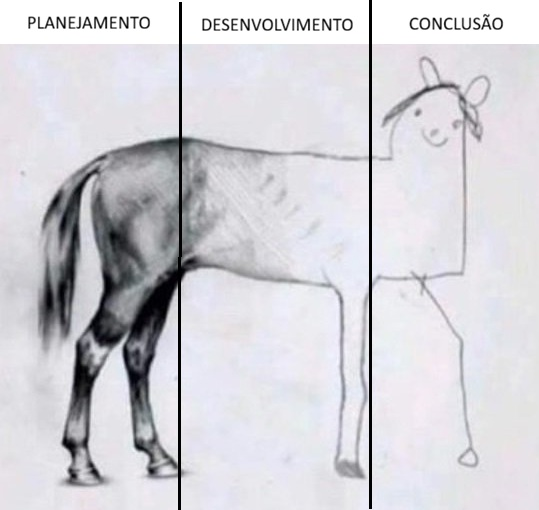
\includegraphics[keepaspectratio]{imagens/pesquisa_cientifica.jpg}}

}

\caption{\label{fig-pesquisa}Etapas do desenvolvimento da pesquisa
científica.}

\end{figure}%

\subsection*{Tables}\label{tables}
\addcontentsline{toc}{subsection}{Tables}

\pagebreak
\newpage

\section*{Apendices}\label{apendices}
\addcontentsline{toc}{section}{Apendices}

\section*{Non-used figures and
tables}\label{non-used-figures-and-tables}
\addcontentsline{toc}{section}{Non-used figures and tables}

\begin{tcolorbox}[enhanced jigsaw, breakable, left=2mm, rightrule=.15mm, opacitybacktitle=0.6, colbacktitle=quarto-callout-warning-color!10!white, arc=.35mm, toprule=.15mm, colframe=quarto-callout-warning-color-frame, leftrule=.75mm, bottomtitle=1mm, toptitle=1mm, titlerule=0mm, title=\textcolor{quarto-callout-warning-color}{\faExclamationTriangle}\hspace{0.5em}{Non-used codes}, colback=white, bottomrule=.15mm, opacityback=0, coltitle=black]

\end{tcolorbox}




\end{document}
